\documentclass[wide,a4paper,titlepage,12pt] {article}
\usepackage{polski}
\usepackage[utf8]{inputenc}
\usepackage{listings}
\usepackage{float}
\usepackage{slashbox}
\usepackage[table]{xcolor}
\usepackage{graphicx,pdflscape}
\usepackage{placeins}


\title{Grafika komputerowa}
\author{Tymon Tobolski (181037)}

% Title page layout (fold)
\makeatletter
\renewcommand{\maketitle}{
\begin{titlepage}
  \begin{center}
    \vspace*{3cm}
    \LARGE \@title \par
    \vspace{2cm}
    \textit{\small Autor:}\par
    \normalsize \@author\par \normalsize
    \vspace{3cm}
    \textit{\small Prowadzący:}\par
    Dr inż. Tomasz Kapłon \par
    \vspace{2cm}
    Wydział Elektroniki\\ III rok\\ Pn TP 08.15 - 11.00\par
    \vspace{4cm}
    \small 14 listopada 2011
  \end{center}
\end{titlepage}
}
\makeatother
  \lstset{
    language=c++,
    basicstyle=\ttfamily\scriptsize,
    numbers=left,
    numberstyle=\scriptsize,
    stepnumber=10,
    numbersep=9pt,
    showspaces=false,
    showstringspaces=false,
    showtabs=false,
    breaklines=true,
  }

\begin{document}
\maketitle
  \section{Cel laboratorium}
  \paragraph{}
  Celem laboratorium była prezentacja obiektów trójwymiarowych w rzucie perspektywicznym oraz realizacja prostej interakcji z użytkownikiem polegającej na sterowaniu ruchem obiektu i położeniem obserwatora w przestrzeni 3-D za pomocą myszy.

  \section{Obrót obiektu}
  \paragraph{}
  Program wyświetla czajnik i pozwala na jego obrót za pomocą myszy. Po wciśnięciu lewego przycisku myszy i przesunięciu kursora w lewo lub w prawo czajnik obraca się wokół osi Y, natomiast przesunięcie kursora w górę lub w dół ekranu powoduje obrót obiektu wokół osi X. Ponadto wciśnięcie prawego przysiku myszy pozwala na przybliżanie lub oddalanie obiektu poprzez przesuwanie kursora w pionie.

  \paragraph{}
  \lstinputlisting{1.cpp}

  \newpage
  \begin{figure}[h!]
    \begin{center}
      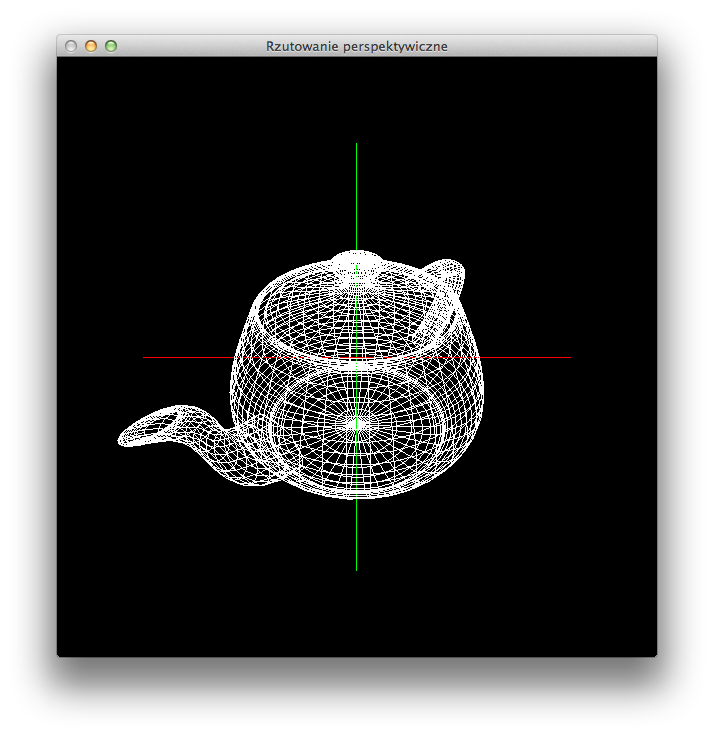
\includegraphics[width=\textwidth]{1.png}
      \caption{Czajnik obrócony wokól osi X i Y}
    \end{center}
  \end{figure}

  \newpage

  \section{Sterowanie położeniem obserwatora}
  \paragraph{}
  W tym zadaniu zamiast czajnika wykorzystane zostało jajko z poprzedniego laboratorium. Program umożliwia zmiane położenia obserwatora za pomocą myszy. Przesuwanie kursora w pionie i w poziomie (wraz z wciśniętym lewym przyciskiem myszy) zmienia odpowiednie kąty określające pozycje obserwatora. Podobnie jak w zadaniu poprzednim przesuwanie kursora z wciśniętym prawym klawiszem myszy powoduje zoom obiektu.
  \newpage
  \begin{figure}[h!]
    \begin{center}
      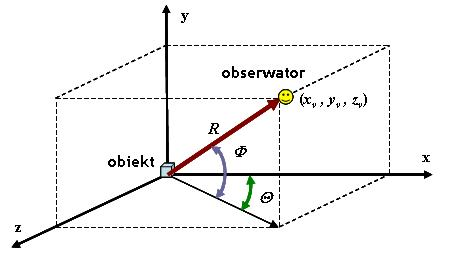
\includegraphics[width=\textwidth]{3.jpg}
      \caption{Położenie obserwatora względem obiektu}
    \end{center}
  \end{figure}


  \paragraph{}
  \lstinputlisting{2.cpp}

  \begin{figure}[h!]
    \begin{center}
      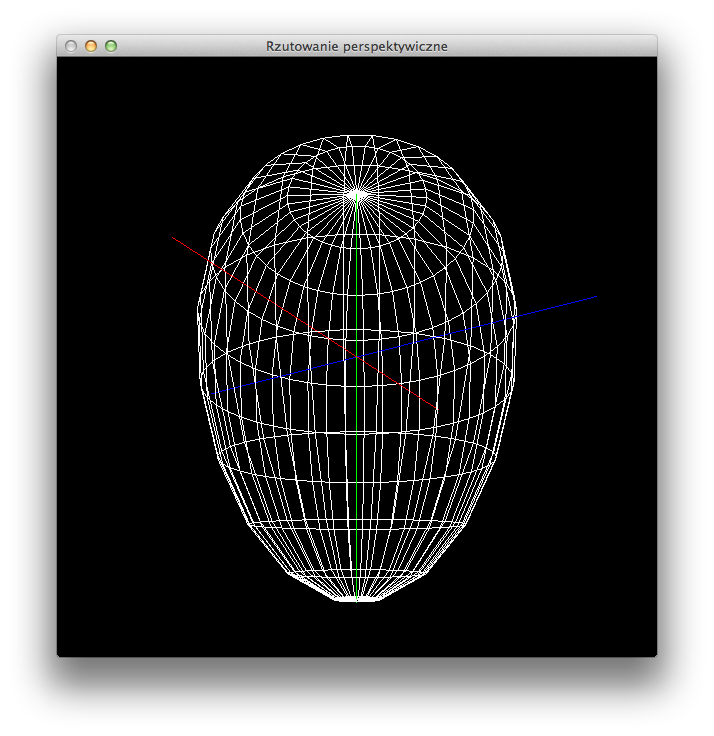
\includegraphics[width=\textwidth]{2.png}
      \caption{Zmiana położenia obserwatora}
    \end{center}
  \end{figure}

  \section{Wnioski}
  \paragraph{}
  Wszystkie zadania zostały zrealizowane w czasie laboratorium. Największe trudności sprawiło przejście przez punkt krańcowy przy obrocie w zadaniu 2. Miało to związek z charakterystyką funkcji $sin$. Rozwiązaniem okazało się ograniczenie kąta $\Phi$ do wartości z przedziału $<-\pi ; \pi>$, a następnie zmiana położenia obserwatora poprzez parametr funkcji $gluLookAt$ w zależności od strony, na którą "patrzy" obserwator.


\end{document}